\chapter{Formalism}\label{chap:Formalism}

This chapter introduces the reader to the more rigorous concepts and mathematical background that will required to fully understand the material presented in the later chapters of this dissertation. 

A discussion of multiplexing and signal-to-noise ratio will be discussed, as well are various coding schemes used in various notable computational sensors as well as the ones in this disseration. 


The vast majority of modern optical sensing involves an \acrfull{adc} step, which creates discrete digital values from a physical phenomena. Therefore, we will concentrate on continuous-to-discrete and discrete-to-discrete measurements. This not only makes the formalism we will discuss more relavent but in many cases it will simplify the mathematics. 

As described earlier in \Cref{chap:Introduction}, a \gls{measurement} is a map from the physical signal-of-interest \gls{objvec} to the measurement data \gls{measvec}. The solutions to the electromagnetic wave equation are linear in free space so the propagation of electromagnetic radiation is linear. We can also approximately model the response of our sensors as linear. Thus we can write the measurement as an integral
%
\begin{equation}
	g_m = \int \mb{f}( \mb{x} ) h_m ( \mb{x} ) d \mb{x}
\end{equation}
%
where $ h_m ( \mb{x} ) $ is the continuous-to-discrete measurement process from point $ \mb{x} $ to discrete measurement index \gls{m}. We can write the continuous signal-of-interest as a superposition over a basis 
%
\begin{equation}
	f( \mb{x} ) = \sum_{n} f_n \psi_n ( \mb{x} )
\end{equation}
%
This allows us to express the measurement of any optical phenomena as a matrix multiplication
%
\begin{equation}
\mathbf{g} = \mathbf{Hf}
\label{eq:gHf}
\end{equation}
%
where \gls{measvec} is now a measurement data vector and \gls{objvec} is the discrete representation of the object signal-of-interest and $\mb{H}$ is the matrix which describes measurement process. For brevity we will refer to the \gls{objvec} as the object and $\mb{H}$ as either the sensing matrix or the measurement matrix. \Cref{eq:gHf} represents the forward model in a wide variety of computational sensors. The object \gls{objvec} is a vector in \gls{n} dimensional vector space and the measurement \gls{measvec} is a vector in \gls{m} dimensional vector space. In general $m \neq n$. Note that \Cref{eq:gHf} is an extremely useful way to represent the forward model in optics, since it allows us invoke a vast amount of computationally attractive numerical techniques which are dedicated to linear systems.

In the real-world noise degrades the measurements 
\begin{equation}
	\mb{g}=\mb{Hf} + \mb{e}	
\end{equation}
where \gls{noisevec} is additive noise. Additive noise is noise which is independent of the signal. An example of additive noise includes the thermal noise generated by the random fluctuations of the charge carriers from \gls{ccd} electronics. A different type of noise called multiplicative noise also exists, but will not be considered in this dissertation. 

\section{Isomorphic Sensing}

In an isomorphic measurement, where the goal is a one-to-one mapping of object points to measurement points, the measurement matrix is often modeled with the identity matrix
\begin{equation}
	\mb{H}=\mb{I}	
\end{equation}


We can get an idea of how much error exists in an isomorphic measurement through invoking the weighing example again. This example was originally discussed in book \cite{harwit2012hadamard} but it is so useful in the context of this dissertation I will briefly summarize it here. In the weighing example, let's say we have $4$ objects with true unknown weights $f_{1}, f_{2}, \cdots, f_{4}$. We record the measured weights $g_{1}, g_{2}, \cdots, g_{4}$ with additive noise (random error)  $ e_1, e_2, \cdots, e_4 $. The forward model with noise is 
\begin{equation}
	\left[ \begin{matrix} g_1\\ g_2\\ g_3\\ g_4\end{matrix} \right] = \left[ \begin{matrix} 1& 0& 0& 0\\ 0& 1& 0& 0\\ 0& 0& 1& 0\\ 0& 0& 0& 1\end{matrix} \right] \left[ \begin{matrix} f_1\\ f_2\\ f_3\\ f_4\end{matrix} \right] + \left[ \begin{matrix} e_1\\ e_2\\ e_3\\ e_4\end{matrix} \right] 
	\label{eq:gHfpluse}
\end{equation}
The estimated weights \gls{estobjvec} are the measurements  $ \mathbf{g} $
\begin{equation}
	\mathbf{ \hat{ f }} = \mathbf{g} 
\end{equation}
Where the error between the estimated weights and the actual weights is the error $ \mb{n} = \mbh{f} - \mb{f} $. For our purposes the assumption of a zero mean distributed noise is a good assumption. This allows us to assume the the isomorphic measurements are unbiased. For an unbiased estimator, the mean squared error of the estimated weight is the variance
\begin{equation}
	E [ ( \mb{e} )^2 ] = E [ ( \mbh{f} - \mb{f} )^2 ] = \sigma^2.
\end{equation}
The smallest possible mean square error is limited to the variance of the noise. Now, I will show how multiplexing codes can be used to reduce the mean square error of the estimate. 

\section{Multiplexing}

As we discussed in \cref{chap:Introduction}, \gls{multiplexing} is an extremely useful technique for overcoming trade-offs in traditional optical sensing. Now it is time to discuss and demonstrate the quantitative advantages provided by multiplexing. 

In a multiplexed measurement, each element in the measurement vector \gls{measvec} is a weighted linear combination of the elements in the object vector. Therefore the measurement matrix $\mb{H}$ is no longer an identity matrix. 



\subsection{Coding Schemes}\label{subsec:codingschemes}

We will now discuss formally the properties, advantages and disadvantages of several popular multiplex coding schemes used in computational sensing especially in dispersive spectroscopy such as the Hadamard, S-Matrices, and random coding. 

A Hadamard matrix of order $n$ is defined as a matrix \gls{hadamardn} as the $n \times n$ matrix whose elements consist of $+1$'s and $-1$'s and satisfies the following property:
\begin{equation}
	\mb{H}_{n}^T \mb{H}_{n} = \mb{H}_{n} \mb{H}_{n}^T = n I_{n}
\end{equation}
where $\mb{I}_n$ is an $n \times n$ indentity matrix. 

In multiplex spectroscopy and imaging, Hadamard codes are extremely popular for a variety of reasons. Hadamard codes are provably optimal in the case where we are allowed to take a full set of measurements, meaning that \gls{objvec} and \gls{measvec} from \cref{eq:gHf} are both vectors in $n$ dimensional space and when one uses both $+1$'s and $-1$'s in the code \cite{harwit2012hadamard}.  In this case, Hadamard codes achieves the minimal the mean square error defined as
\begin{equation}
	\text{MSE} = \frac{1}{n} ( e_1 + e_2 + \cdots e_n )^2 
\end{equation}

In the weighing example, we can get negative measurements by using a balancing scale instead of a spring scale. An Hadamard multiplexed measurement would look like
\begin{equation}
\left[ \begin{matrix} g_{1}\\ g_{2}\\ g_{3}\\ g_{4}\end{matrix} \right] =\left[ \begin{matrix} +1 +1 +1 +1 \\ +1 -1 +1 +1 \\ +1 -1 -1 +1 \\ +1 -1 -1 +1 \end{matrix} \right] \left[ \begin{matrix} f_{1}\\ f_{2}\\ f_{3}\\ f_{4}\end{matrix} \right]
\end{equation}
This means that in the first measurement all 4 items at placed in the same pan. In the second measurement items 1 and 3 are in the same pan while items 2 and 4 are in the opposite pan, etc \cite{harwit2012hadamard}. We have four equations and four unknowns so we can solve for the estimates using algebra

\begin{align*}
  \hat{f}_1 &= \frac{1}{4} (g_1 + g2 + g2 +g4) \\
  &= f_1 + \frac{1}{4}(e_1 + e2 + e3 + e4) \\
        \mathrel{\makebox[\widthof{=}]{\vdots}} \\
  \hat{f}_4 &= \frac{1}{4} (g_1 - g2 - g2 +g4) \\
  &= f_4 + \frac{1}{4}(e_1 - e2 - e3 + e4)
\end{align*}
The mean square error of the $m^{th}$ measurement  
\begin{equation}
	E [ ( \hat{f}_{m} - {f}_{m} )^2 ] = \frac{1}{4} \sigma^2.
\end{equation}
which is $4$ times lower than using an isomorphic measurement scheme. In general, the \gls{mse} of a Hadamard measurement is 
\begin{equation}
	\text{MSE} = \frac{\sigma^2}{N_{\lambda}}
	\label{eq:hadamardmse}
\end{equation}
where \gls{numspecchan} is the number of spectral channels, which is equal to the number of measurements \gls{nummeas}. Hotelling proved in 1944 that for a measurement matrix with elements $h_{mn} \in [-1, +1]$ the lowest possible MSE for the case of a full set of measurements is with a linear unbiased estimator is $\text{MSE} = \frac{\sigma^2}{N_m}$ \cite{brady2009optical}. So, one cannot possibly do better than Hadamard coding in this case. We will see later in other special cases that we can beat Hadamard codes.

In many practical cases in computational sensing, making a code with simultaneous positive and negative modulation of the signal is not possible. For incoherent light, the response is linear in intensity. In the case where one has the ability to make a full set of measurements but is limited to elements of $+1$'s and $0$'s, an S-Matrix code minimizes the \gls{mse} \cite{harwit2012hadamard}.

In the weighing example, a spring balance rather than a two pan scale analogous to this situations. 
\begin{equation}
\left[ \begin{matrix} g_{1}\\ g_{2}\\ g_{3}\\ g_{4}\end{matrix} \right] = 
\left[ \begin{matrix} 0 & +1 & +1 & +1 \\ +1 & +1 & 0 & 0 \\ +1 & 0 & +1 & 0 \\ +1 & 0 & 0 & +1 \end{matrix} \right]
\left[ \begin{matrix} f_{1}\\ f_{2}\\ f_{3}\\ f_{4}\end{matrix} \right]
\end{equation}
So items 2, 3, and 4 are weighed together, then 1 and 2, and so on. Solving the system of equations in a silimar fashion as before in the Hadamard weighing example we find that the mean square error for the $m^{th}$ measurement when weighing 4 items is 
\begin{equation}
\text{MSE} = E [ ( \hat{f}_{m} - {f}_{m} )^2 ] = \frac{7}{9} \sigma^2.
\end{equation}
Which reduced the \gls{mse} compared to the isomorophic measurement scheme but it is less of a reduction compared to the Hadamard measurement scheme. The \gls{mse} of the S-Matrix is approximately a factor of 4 increase compared to the Hadamard matrix coding scheme. 

In the case when the full set of measurements are availible, random coding schemes are provably sub-optimal to compared to Hadamard and S-Matrix codes. However, they should not be ignored because in compressive sensing, certain theoretical garuntees exist for random coding that do not exist for Hadamard and S-Matrix codes. Sometimes, the physics of the situation forces a random coding scheme. There is little literature on the performance of random coding schemes. At the time of this writing (2016), I am unaware of an optimality proofs for random codes when one has a full set of measurements availible. 

\subsection{The Fellgett Advantage}

The \gls{Fellgett advantage} is the improvement in \gls{snr} that occurs when an instrument takes multiplexed measurements compared to isomorphic measurements \cite{fellgett1958principes, davis2001fourier}. Physically the \gls{Fellgett advantage}  occurs because a single detector element produces a noise contribution whether it's sampling a single part of the object or multiple parts of the object. Maximizing the \acrfull{snr} of the estimated object signal-of-interest for a given system throughput and detector noise is major design consideration in computational optical sensing particularly in the area of spectroscopy. In spectroscopy, there are two well known multiplex schemes, the Hadamard multiplexing in dispersive spectrometers and the interferometric spectrometer . 

The \gls{fts} architecture is a similar to the Michelson interferometer, see Figure \ref{fig:fourierTransformSpec}.The \gls{fts} operates by taking the autocorrelation of the complex electric field as a function of time delay by moving one of the mirrors in the interferometer \cite{davis2001fourier}. The Wiener-Khinchin theorem says that for a wide-sense stationary random process, the Fourier transform of the autocorrelation is the power spectral density. Thus a computational post-processing step is required to reconstruct the spectrum from the measurement data. Since the \gls{fts} measures combinations of multiple wavelengths at each detector readout it also exhibits the \gls{Fellgett advantage}.

The advantage that multiplexing provides over an isomorphic measurement depends on the coding sceheme. We've just seen that for a Hadamard coding scheme the \gls{mse} is given by \Cref{eq:hadamardmse}. It turns out that for a \gls{fts} the \gls{mse} obtained is a factor of two greater than the Hadamard multiplexing scheme \cite{tai1976fourier}. 

\begin{equation}
	\text{MSE} = 2 \frac{\sigma^2}{N_{\lambda}} 
\end{equation}


\begin{figure}
	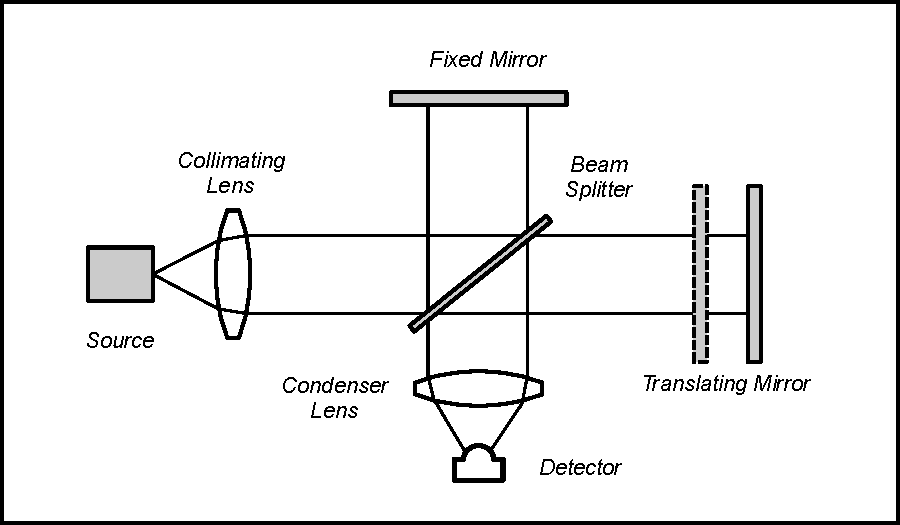
\includegraphics[scale=1]{fourierTransformSpec}
	\captionof{figure}[The architecture of the Fourier Transform Spectrometer.]{The architecture of the Fourier Transform Spectrometer resembles the Michelson interferometer. One of the mirrors is translated back and forth. The interferogram is the detected intensity versus mirror delay which is related to the autocorrelation of signal. The Fourier transform of the autocorrelation provides the spectrum.}
	\label{fig:fourierTransformSpec}
\end{figure}


\section{Principal Component Analysis}

Principal component analysis (PCA) is a technique that attempts to recast a dataset in manner which allows us to maximally discriminate the data with just a few vectors. The first vector points in the direction of maximum variance. The second vector points in a direction that also maximizes variance but is orthogonal to the first vector and so on. These new vectors are called the \emph{principal components}. We will say the \emph{rows} of matrix $\mb{P}$ are the principal components. 

Let's say we have a dataset $\mb{S}$ which consists of $N$ spectra with \gls{numspecchan} spectral channels. Instead of looking at the data as just intensity versus spectral channel, \gls{pca} attempts to construct a set of new vectors (also called features) that show as much variation in the spectra as possible. In other words, first direction (principal component) is used to recast the data to look as different (uncorrelated) as possible. This allows us to discriminate the data, as best we can with just one direction. The second principal component is the direction that provides the second most ability to discriminate the data, and so on. 

The covariance matrix is defined as
\begin{equation}
\mb{C_{X}} = \frac{1}{N} \mb{S} \mb{S}^{T}.
\end{equation}
Each element in the covariance matrix $C_{Xmn}$ is the covariance of the $m^{th}$ spectrum $\mb{s}_m$ and the $n^{th}$ spectrum $\mb{s}_n$. 
\begin{equation}
C_{Xmn} = \frac{1}{N} \mb{s}_m \mb{s}_n^{T}.
\end{equation}

Note that large covariance means they look quite alike and therefore are difficult to disambiguate.

If the entire collection of spectra $\mb{S}$ were mutually orthogonal, being able to tell one spectrum apart from another would be easy. You would just have a collection of spikes at different spectral channels. The covariance matrix in this case would be a diagonal matrix. 

Since there is typically some redundancy between spectra, the off-diagonal elements of the covariance matrix will be non-zero. The principal components allow us to recast the data to make it as uncorrelated as possible in a new basis. 
\begin{equation}
	\mb{Y} = \mb{PX}
\end{equation}
where $\mb{Y}$ is the data projected onto the principal component basis $\mb{P}$. The covariance of the projected data
\begin{equation}
	\mb{C_{Y}} = \frac{1}{N} \mb{Y} \mb{Y}^{T} 
\end{equation}
is a now diagonal matrix. Indeed, the principal components are the optimal way to discriminate the spectra in the dataset \cite{}.

It turns out there is a way to calculate the principal components in closed form. The \emph{eigenvectors of the covariance matrix are the principal components} \cite{shlens2014tutorial}. 

Since the full set of principal components forms a basis, each spectra $\mb{s}$ in $\mb{S}$ can be written as a superposition of principal components without any error
\begin{equation}
\mb{s} = \sum_{\lambda = 1}^{N_{\lambda}} y_{\lambda} \mb{v}_{\lambda}
\end{equation}
In many cases, only a few of the first principal components are needed in the summation to approximate the original data well.
\begin{equation}
{\mb{s}} \approx \sum_{\lambda = 1}^{M} y_{\lambda} \mb{v}_{\lambda}
\end{equation}
Where $M \ll N_{\lambda} $. Note that each eigenvector has an associated eigenvalue. The eigenvalues are also informative because they can tell us how many principal components are really needed to discriminate all of the spectra. The magnitude of the eigenvalue tells us how well it's associated eigenvector is at discriminating the data.

This is another reason why \gls{pca} is so useful. It can be used as a type of lossy compression code and as a measurement matrix for compressive sensing. Simply project the data onto the first several principal compoenents associated with the largest $M$ eigenvalues. 

The \gls{afssi-c} relies on a variation of Principal Component Analysis (PCA) for discriminating between spectra. In addition to \gls{pca} the AFSSI-C uses a Bayesian probability to create adaptive codes. We will now discuss some of fundamentals of Bayesian probability and the Log-likelihood ratios. 

\section{Bayesian statistics and Maximum a Posteriori}

In the real world, measurements are corrupted by noise. The random nature of noise corrupted measurements lends itself to a stochastic perspective of signals. A hypothesis can be associated with various parameters or aspects of a signal. A hypothesis is nothing more than a claim or premise that one is interested in verifying. In imaging and spectroscopy, one example is that at a certain location in the field of view, the hypothesis is that a spectrum is present or not present. Another hypothesis is that the mean value of the signal is some value. Instead of attempting to determine whether a hypothesis is true, often times we are interested in estimating parameters of stochastic processes, which we denote $\theta$.

Bayesian statistics allows one to treat the hypothesis or parameters as random variables rather than deterministric constants. A wide variety of Bayesian approaches exist and each require a heavy reliance on Bayes's theorem. Bayes' theorem is a way of computing probabilities of a hypothesis given some evidence which are related to the hypothesis. For example, Bayes' theorem can be used to decide which of two bags of candy has been opened or if a spectrum is present. The idea is that we can make a more informed calculation of probability if we are able to account or update the probability given some new piece of evidence that we may have not had at the beginning.

The derivation of Bayes' theorem follows from the definition of conditional probability, the conditional probability of event $A$ occuring given that $B$ occured is:

\begin{equation}
	P \left( A \given[\big] B \right) = \frac{ P \left( A \cap B \right) }{ P \left( B \right)}
\end{equation} 
this can be seen graphically in Figure


\begin{figure}
	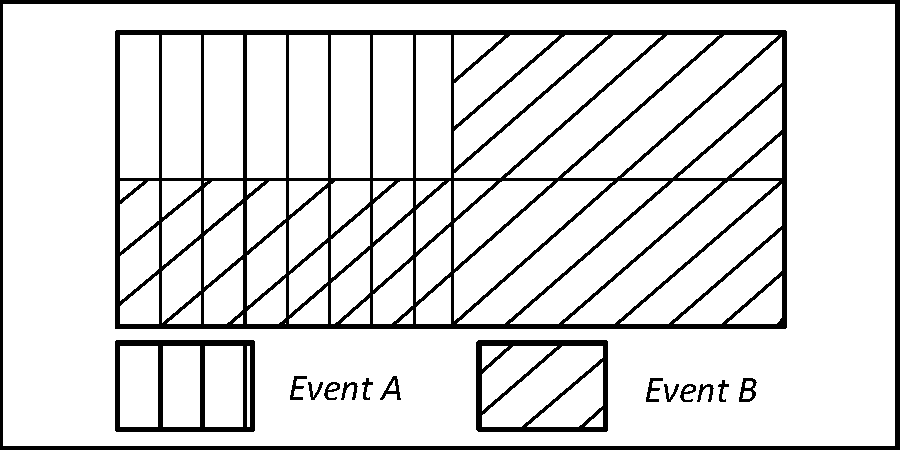
\includegraphics[scale=1]{definitionOfConditionalProbability}
	\captionof{figure}[Graphical demonstration of joint probability.]{Graphical demonstration of joint probability. The probability of event $A$ is $P(A)=3/4$. The probability of event $B$ is $P(B)=3/4$. The joint probability of events $A$ and $B$ is $P(A \cap B) = 1/4$. The probability of event $A$ occuring given that event $B$ has occured is $P( A \given B) = 1/3$. This is consistent with the equation $ P(A \cap B) = P(A \given B) P(B) $}
	\label{fig:definitionOfConditionalProbability}
\end{figure}

solving for the joint probability $ P \left( A \cap B \right) $ gives
\begin{equation}
 P \left( A \cap B \right) =	P \left( A \given[\big] B \right)  P \left( B \right)
\label{eq:bayeStep2}
\end{equation} 
since the joint probability commutes $ P \left( A \cap B \right) = P \left( B \cap A \right) $, we can also write
\begin{equation}
 P \left( A \cap B \right) =	P \left( B \given[\big] A \right)  P \left( A \right)
\label{eq:bayeStep3}
\end{equation} 
equatin the right hand side of Equation \ref{eq:bayeStep2} and Equation \ref{eq:bayeStep3} gives use Bayes' theorem (also called Bayes' rule)
\begin{equation}
	P \left( A \given[\big] B \right) = \frac{ P \left( A \right) P \left( B \given[\big] A \right) }{ P \left( B \right) }
\end{equation}

One interpretation of Bayes' theorem is called the Diachronic interpretation, which says that conditional probability of the hypothesis or parameter $\theta$ given knowledge of some evidence or measurement data $g$ is given by 

\begin{equation}
	P \left( \theta \given[\big] g \right) = \frac{ P \left( \theta \right) P \left( g \given[\big] \theta \right) }{ P \left( g \right) }
	\label{eq:diachronic}
\end{equation}

The term $ P \left( \theta \given[\big] g \right) $ is called the posterior. It represents our belief in the hypothesis given the data. The term $ P \left( \theta \right) $ is called the prior. $P \left( g \given[\big] \theta \right)$ is called the Likelihood. $P \left( \theta \right)$ is called the normalizing constant. In general the normalizing constant can be written as 
\begin{equation}
P \left( \theta \right) = \sum_{i} P \left( \theta_i \right) P \left( g_i \given[\big] \theta_i \right)
\label{eq:normalizingConstant}
\end{equation}
One can repeatly apply Bayes' theorem given new measurement data. We will use a simple example to illustrate how to update the belief. Imagine we have two bags of candy. Bag 1, which we denote $B_1$, has 10 pieces of cherry flavored candy, denoted as $C$, and has 30 pieces of strawberry flavored candy, denoted as $S$. Bag 2, $B_2$, has 20 pieces of cherry candy and 20 pieces of strawberry candy. At the beginning, the prior probability of selecting bag 1 or bag 2 is both equal
\begin{equation}
	P \left( B_1 \right) = P \left( B_2 \right) = \frac{1}{2}
\end{equation}
Someone then picks a bag at random and takes out a piece of candy that turns out to be strawberry flavor. What is the probability that bag 1 was selected? We can use Bayes' theorem to compute this

\begin{equation}
	P \left( B_1 \given[\big] S \right) = \frac{ P \left( B_1 \right) P \left( S \given[\big] B_1 \right) }{ P \left( S \right) }
\end{equation}

Where $ P \left( S \given[\big] B_1 \right) $ means the probability of selecting a strawberry candy assuming we have selected bag 1, which is $3/4$. The $ P \left( S \right) $ is the probability of selecting a strawberry candy from either bag 1 or bag 2, which $5/8$. Thus

\begin{equation}
	P \left( B_1 \given[\big] S \right) = \dfrac {\left( \dfrac {1} {2}\right) \left( \dfrac {3} {4}\right) } {\left( \dfrac {5} {8}\right) } = \frac{3}{5}
\end{equation}
Similarly, the probability that the person chosen bag 2 is $P \left( B_2 \given[\big] S \right) = 2/5$. Qualatatively, this makes sense, since bag 1 contained more strawberry flavored candy, the belief that bag 1 was chosen should increase and the belief that bag 2 was not chosen should decrease.

Now let's continue the example. Say we put the first piece of candy back in the bag and draw another piece of candy, which turns out to be cherry flavor. Now we must update the beliefs with this new piece of information. We can keep using Baye's theorem, but the trick is that the posterior from the last draw is now used as the prior for the current update.

\begin{equation}
	P \left( B_1 \given[\big] C \right) = \frac{ P \left( B_1 \given[\big] S \right) P \left( C \given[\big] B_1 \right) }{ P \left( C \right) }
\label{eq:updatedBayes1}
\end{equation}

\begin{equation}
	P \left( B_2 \given[\big] C \right) = \frac{ P \left( B_2 \given[\big] S \right) P \left( C \given[\big] B_2 \right) }{ P \left( C \right) }
\label{eq:updatedBayes2}
\end{equation}

The probability of drawing a cherry flavored candy assuming bag 1 was chosen is $ 1/4$ and the probability of drawing a cherry flavored candy assuming bag 2 was chosen is $1/2$. We now must use Equation \ref{eq:normalizingConstant} to compute the normalizing constant, otherwise the posterior probabilities will not sum to 1. In this case $ P(C) = 7/20 $. Plugging these numbers into Equations \ref{eq:updatedBayes1} and \ref{eq:updatedBayes2} gives the updated posterior probabilities

\begin{equation}
	P \left( B_1 \given[\big] C \right) = \frac{3}{7} \approx 0.43
\end{equation}

\begin{equation}
	P \left( B_2 \given[\big] C \right) = \frac{4}{7} \approx 0.57
\end{equation}

Intuitively, drawing a cherry flavored candy has reduced our belief that bag 1 was chosen since bag 1 consist of only $1/4$ cherry flavor candies while bag 2 consisted of $1/2$ cherry candy. 

Sometimes one is given a set of possible parameters that we are interested in estimating, $ \mb{\theta} $, given some measurement data $ g $. The method of \acrfull{map} says the parameters  $ \mb{\theta} $ which maximize the posterior probability are the most likely parameters. 

\begin{equation}
	\mb{\theta}_{map} = \argminA_{\mb{\theta}} \: p\left( \mb{\theta} \given[\big] g \right) 
	\label{eq:map}
\end{equation} 
Using Bayes' theorem we can rewrite Equation \ref{eq:map} as 
\begin{equation}
	\mb{\theta}_{map} = \argminA_{\mb{\theta}} \: \frac{ p\left( g  \given[\big] \mb{\theta} \right) p\left( \mb{\theta} \right) } { p\left(  g \right) }
\end{equation} 
Maximizing the posterior is now equal to maximizing the likelihood and prior. In certain cases, one needs to decide between two sets of parameters or hypotheses. One can do an analogous technique of comparing the posteriors by using a ratio

\begin{equation}
	\frac{ p( \theta_i | g ) }{ p( \theta_j | g ) } = \frac{ p(g|\theta_i) }{ p(g|\theta_j)} \frac{p(\theta_i)}{p(\theta_j)}
\end{equation}
If the ratio is larger than some threshold value then one choses parameter $\theta_i$ and if the ratio is less than the threshold then one choses $\theta_j$. Similar to the earlier example of updating the posterior based on new data, one can update the \gls{map} decision based on new data. Define the likelihood ratio of the $m^{th}$ measurement as 
\begin{equation}
	\Lambda_m = \frac{ p(g_m|\theta_i) }{ p(g_m|\theta_j)}
\end{equation}
After each new set of measurement data $g_{m}$ is collected, one can update the posterior ratios by multiplying the likelihood ratio from the old set of data with the likelihood ratio of the new set of data. The ratio which includes all the updates from measurement $m = 1$ to measurement $m = N_m$ is written as
\begin{equation}
	\frac{ p( \theta_i| \{ g \} _{N_m} ) }{ p( \theta_j | \{ g \} _{N_m} ) } = \displaystyle\prod_{m=1}^{N_m} \Lambda_m \frac{p(\theta_i)}{p(\theta_j)}
\end{equation}
where the notation $\{ g \} _{N_m}$ represents the set of all data from measurement $m$ to $N_m$.

Bayesian statistics is a useful way to update one's belief in a hypothesis or estimate a set of parameters. The Bayesian perspective is a different from the classical perspective. A classical approach to statistical estimation views parameters of interest as deterministic but unknown constants. The Bayesian approach assumes that $\theta$ is a random variable whose particular realization we must estimate.

As we've just seen through the Bayesian approach, the ability to take advantage of new measurement data and prior knowledge is a powerful concept. We will continue on this theme as we discuss \gls{compressive sensing} which relies heavily on the prior assumption of \gls{sparsity}.

\section{Compressive Sensing}

The fundamental approach of \gls{compressive sensing} is that rather than sampling at a high rate and then compressing the sampled data, one can dramatically reduce the number of samples by sampling the signal in a compressed form. I will now discuss some of the more formal concepts of compressive sensing and some techniques to compressively sampling signals. This allows one to build some intuition about compressive sensing. In order to understand why compressive sensing is so powerful we should first discuss the conventional sampling strategy.


\subsection{The Nyquist-Shannon Sampling Theorem}

One of the most important results concerning the \gls{sampling} of continuous signals is the Nyquist-Shannon sampling theorem (often referred to as the \emph{sampling theorem} for short). The sampling theorem says that exact reconstruction of a continuous \gls{bandlimited signal} $f(x)$ is possible if the sampling frequency $f_s$ is atleast twice the maximum frequency $ B $ of the signal \cite{shannon1949communication}. Assuming that a bandlimited signal $f(x)$ has been sampled according to the sampling theorem, then exact recovery from the discrete samples $f_n$ is guaranteed.

However, if the sampling frequency is less than twice the maximum bandwidth $f_s < 2B$, then aliasing may occur in the reconstruction. Aliasing is the effect that high frequencies in the original signal will represented as lower frequencies after reconstruction and information contained in the high frequencies will be potentially lost \cite{proakis1988introduction}. 

Before we continue, it's important to clarify a small but important distinction between the meaning of \gls{sampling} and the meaning of a \gls{measurement}. A measurement is any process that maps physical phenomena which contains a signal-of-interest into measurement data. The measurement data may or may not be discrete. Sampling has a more precise mathematical definition. It is the process of mapping a continuous signal into a sequence of discrete numbers which are called the samples. 

\subsection{Sparsity, Incoherence, and the Restricted Isometry Property}

At first glance, \gls{compressive sensing} seems to go against the Nyquist-Shannon sampling theorem, however the sampling theorem's guarantee of exact reconstruction of a continuous signal relies on the assumption of a bandlimited signal and uniform periodic sampling, which leads to isomorphic sampling. \Gls{compressive sensing} makes different assumptions:  \gls{sparsity} and \gls{incoherence}. Combined with non-linear optimization techniques, \gls{compressive sensing} allows one to take far less samples without significant loss of information. Before we discuss how to actually do compressive sensing and some of its drawbacks, it is important to have a formal discussion of these concepts.

Most continuous signals $f(x)$ can be writen as a discrete summation of orthonormal basis functions
\begin{equation}
	f(x) = \sum_{n=1}^{N} a_n \Psi_n(x),
	\label{eq:expansionEquation1}
\end{equation}
where $a_n$ are the coefficients. I will call the vector $\mb{a} = [ a_{1} \: a_{2} \: \dots \: a_{N} ]^T$ the representation vector of the signal and $\mb{\Psi}$ the representation basis. This allows us to rewrite the signal as a matrix multiplication
\begin{equation}
	\mb{f} = \mb{\Psi}\mb{a}.
\end{equation}

As we discussed in \Cref{chap:Introduction}, any vector $\mb{a}$ is \gls{sparse} when all but a few of its entries are zero. A vector is called $K$-sparse when it has at most $K$ non-zero entries. In real situations, signals with strictly sparse representation vectors are unlikely. Fortunately, it is possible to have approximately sparse representation vectors, which are called \gls{compressible}. In other words, the sorted magnitudes of the coefficients $|a_n|$ quickly decay. When a signal has an expansion in terms of a compressible representation vector, we can intuitively understand \Cref{eq:expansionEquation1}. Discarding smaller coefficients will not significantly degrade the information in the signal \cite{candes2008introduction}. \footnote{From now on, I will use the words \gls{sparse} and \gls{compressible} interchangeably.} 

The concept of \gls{sparsity} is important in compressive sensing. Sparsity determines how efficiently one can acquire the signals. All things being equal, if $K$ decreases, then the reconstruction error tends to decrease. Sparse representations of the signal are not the only important prequisite for high probability reconstruction.

The random sensing basis is useful because of it's mathematical convience however, we shall show heuristically that incorporating additional prior knowledge of the statistics of the signal can reduce reconstruction error in reconstruction but other computational sensing tasks such as spectral classification. However, the options for compressive sensing bases are still quite limited.

In practice, the signal is sampled in a different basis than the representation basis. For example, while many natural signals have a sparse or compressible representation in various wavelet bases or Fourier bases, sampling using the representation basis is not practical or desirable in many cases. Often a sensing basis \gls{H} is used to perform the sampling. In traditional Nyquist-Shannon sampling, the sensing basis is a collection of delta functions. In compressive sensing for example, the sensing basis is the binary random coded aperture mask in a compressive imaging system \cite{duarte2008single}. In an \gls{lcos} based compressive sensing spectrometer, the sensing basis is a finite set of spectral filters \cite{oiknine2016along, yuan2015compressive}. In short, the representation basis allows a signal to be represented as a sparse vector, while the sensing basis is composed of the functionals that one samples with.

The equation which combines these concepts to model a compressive measurement is

\begin{equation}
	\mb{g} = \mb{H} \mb{\Psi} \mb{a} = \mb{H} \mb{f}
	\label{eq:gHf2}
\end{equation}
where \gls{measvec} is a $N_m \times 1$ measurement vector, \gls{H} is a $N_m \times N$ measurement vector, and $\mb{a}$ is an $N \times 1$ vector. A forward model in compressive sensing obeys \Cref{eq:gHf2} when $N_m \ll N$. 

One important concept in \gls{compressive sensing} is coherence. The coherence between the sensing basis $\mb{H}$ and the representation basis $\mb{\Psi}$ is
\begin{equation}
	\mu \left( \mb{H}, \mb{\Psi} \right) = \sqrt{n} \max_{1 \leq k, 1 \leq n}  | \langle h_k, \psi_j \rangle | ,
	\label{eq:coherenceDef1}
\end{equation}
which defines coherence as a measure of the largest correlation between any two elements of $\mb{H}$ and $\mb{\Psi}$. There is an alternate definition of coherence which is concerned with only the sensing matrix $\mb{H}$ (the sensing matrix is also called the measurement matrix or the system matrix).

\begin{equation}
	\mu \left( \mb{H} \right) =  \max_{k \neq j } \frac{ | \langle h_k, h_j \rangle | } { \left\| h_k \right\|_2 \left\| h_j \right\|_2 }.
	\label{eq:coherenceDef2}
\end{equation}
In this definition, the coherence is the maximum correlation between columns of the system matrix. 

Ideally, one would like to use as less measurements $N_m$ as possible without degrading the reconstructed signal. In \gls{compressive sensing}, the amount of measurements needed is a function of the sparsity and the coherence. Given a coefficient sequence $\mb{a}$ that is $K$-sparse then one needs
\begin{equation}
N_m \geq C \cdot \mu^2 ( \mb{H} , \mb{\Psi} ) \cdot K \cdot \log n
\label{eq:minMeas1}
\end{equation}
for a high probability of reconstruction, where $C$ is just a constant and $n$ is the dimensionality of the original signal.

\Cref{eq:minMeas1} shows the importance of sparsity and coherence in compressive sensing. Lower coherence and sparsity allows one to use less measurements \cite{duarte2008single}. The more incoherent---lower correlation---the two bases are, the higher the probability of succesful reconstruction of compressive measurements. Random matrices have a high probability of being incoherent with any basis \cite{candes2008introduction}. Using the alternate definition of coherence from \Cref{eq:coherenceDef2} produces similar qualitative results \cite{tropp2006just}. 

The isometery constant $\delta_K$ of a matrix \gls{A} $=\mb{H}\mb{\Psi}$ is the smallest number such that 
\begin{equation}
\left( 1 - \delta_K \right) \left\| \mb{a} \right\|_{\ell_2}^{2} \leq \left\| \mb{A} \mb{a} \right\|_{\ell_2}^{2} \leq \left( 1 + \delta_K \right) \left\| \mb{a} \right\|_{\ell_2}^{2} 
\end{equation}
for all $K$-sparse vectors $\mb{a}$. The matrix \gls{A} obeys the \emph{restricted isometry property} (RIP) of order $K$ if $\delta_K$ is not too close to one \cite{candes2008introduction}. If RIP is satisfied, the sensing matrix \gls{A} approximately preserves the Euclidean length of signals. The \gls{rip} is an important theorectical result which allows robust compressive sensing where signals are corrupted by noise. Sensing matrices which have random entries obey the \gls{rip} with high probability \cite{candes2008introduction, duarte2008single, foucart2013mathematical}. 

All of the concepts I have just discussed can be understood at an intuitive level. Sparsity is the idea that the information content of a signal is relatively small compared to the amount of data which originally described the signal. Coherence extends that concept of how invertable a matrix is, the more linearly independent the system of equations, the easier it is to invert the matrix. The restricted isometry property is basically saying that any matrix with a small isometry constant will keep the distance between signal vectors the same. Why is this important? Think of a geometric picture, imagine noise as a sphere of uncertainty around the signal vectors. When the noise is small, two signal vectors can be mapped to a small part of the measurement space and still fit in that space. When one extracts the signal from the measurements, one can tell them apart. As the noise increases one wants the distance between measured signal vectors to at least stay the same and certainly not dramatic decrease, otherwise it will be difficult to tell the signals apart. The \gls{rip} is basically a way of seeing if a measurement matrix will pack the signal vectors with the space distance between them. A small amount of noise will lead to a small amount of reconstruction error instead of a small amount of noise leading to a large reconstruction error. 
\gls{A}


\subsection{Solving Inverse Problems For Compressive Sensing}


I will now discuss inverse problems and several general strategies which allows one to find solutions for the compressive sensing problem when $N_m \ll N$. 

The least squares estimator (LSE) solves the problem of 
\begin{equation}
	\mb{g} = \mb{Ax} + \mb{n}
	\label{eq:gTan}
\end{equation}
by minimizing the objective function 
\begin{equation}
	\argminA_{\mb{x}} \: \sum_{n=1}^{N} \left( \mb{g} - \mb{Ta} \right)^2 = \| \mb{g} - \mb{Ta} \|_{2}^{2}.
\end{equation}
which is the $\ell_2$ norm. The goal is to minimize the square difference between the given data \gls{measvec} and the forward signal model for the data $\mb{Ta}$. There are no probabilistic assumptions about the measurement data. It turns out that a close form version of the LSE exist

\begin{equation}
	\mbh{a} = \left( \mb{A}^T \mb{A} \right)^{-1} \mb{A}^T \mb{g}.
\end{equation}
Alternatively, if the matrix $\mb{A}$ is very large, one may us gradient descent and other convex optimization algorithms to solve the least squares problem. While the \gls{lse} may provide a solution when $N_m \ll N$ these solutions tends to overfit the data in these situations and does not take advantage of the prior knowledge of sparsity in reduce the solution space.

solves \Cref{eq:gHf2} when $\mb{A}$ is linearly independent and when $N_m > N$ then can solve for $\mbh{a}$

The most straight forward technique of estimating or reconstructing a signal from its measurement data given a linear system is through the least squares estimator. 


\begin{equation}\label{eq:lineareq1}
	\mb{g} = \mb{Hr} 
\end{equation}

Given \smb{g} and \smb{H} we want to solve for \smb{r}. If the matrix is full rank then we can simply multiply both sides of equation \ref{eq:lineareq1} by $\mbi{H}$ 



If \smb{H} is not full rank then its inverse does not exist. However we can try to find a solution \smbh{r} that minimizes the least squared error. This is called the \emph{Least Squares Solution} also known as the \emph{Least Squares Estimator}, \emph{Ordinary Least Squares} and by many other names. We define the squared error as

\begin{equation}\label{eq:squarederror1}
	\mathbf{ \lVert \mathbf{e} \rVert }^2 =    \mb{ \lVert \mb{Hr-g} \rVert }^2
\end{equation}

\noindent To minimize the error, we take the derivative of equation \ref{eq:squarederror1} with respect to \smb{r} and set it equal to zero and solve for \smb{r}. The full derivation which shows each step is given in Appendix \ref{app:Derivation of the Least Squares Estimator}. The least squares estimate:

\begin{equation}
	\hat{ \mb{r} } = ( \mbt{H} \mb{H} )^{-1} \mbt{H} \mb{g}
\end{equation}




Given measurements \gls{measvec} and knowledge that $\mb{a}$ is sparse or compressible, solving an optimization problem of the form 
\begin{equation}
	\mbh{a} = \argminA_{\mb{a}} \: \| x \|_{0} \text{\; subject to \;} \mb{Ta} = \mb{g}
	\label{eq:l0min}
\end{equation}
where $\| x \|_{0}$ is the $\ell_0$ norm, which is equal to the number of nonzero entries in vector $\mb{a}$.\footnote{The $\ell_0$ norm is not strictly a norm and is actually a quasi-norm.} \Cref{eq:l0min} return $\mbh{a}$ that resembles $\mb{a}$ as long as the measurement noise is small. This is referred to as $\ell_0$-minimization. The "subject to" constraint ensures the solution agrees with the observed measurement data. Unfortunately, $\ell_0$-minimization is nonconvex which means that iterative methods may not converge to a solution. On the other hand, a convex problem has the property that any local minimum is also a global minimum. It has been shown that for general matrices $\mb{A}$, $\ell_0$- minimization is computationally intractable \cite{aggarwal2007data}. 

Fortunately, one can use practical optimization techniques to find sparse solutions of \label{eq:gTa+e} using
\begin{equation}
	\mbh{a} = \argminA_{\mb{a}} \: \| x \|_{1} \text{\; subject to \;} \mb{Ta} = \mb{g}
	\label{eq:l1min}
\end{equation}
where $\| \mb{a} \|_1 = \sum_{n}^{N}|a_n|$. In other words, \gls{l1}-minimization is a convex problem which allows for fast and accurate reconstruction \cite{foucart2013mathematical}. A more practical version of \Cref{eq:l1min} is written as
\begin{equation}
	\mbh{a} = \argminA_{\mb{a}} \: \| \mb{Ta} = \mb{g} \|_{2}^{2} + \tau \| \mb{a} \|_1
	\label{eq:l1regls}
\end{equation}
where $\tau$ is a non-negative number. \gls{tau} is called the regularization parameter and serves to change the sparsity level of the solution and can be used to account for noise in the vector which increases the robustness of the optimization. In this form, the problem is called $\ell_1$ regularized least squares (LS). $\ell_1$ regularization also appears in the context of basis pursuit denoising \cite{chen2001atomic}. In statistics, $\ell_1$ regularization is used in the LASSO algorithm for feature selection, therefore one often refers to \Cref{eq:l1regls} as the LASSO problem \cite{tibshirani1996regression}. 

 
 is also called Basis Pursu


$  \mathfrak{F} \{ \iint\limits_{a}^{b}  g( \xi, \eta )  h( x - \xi, y - \eta )  d \xi d \eta \}  $

%\bibliographystyle{IEEEtranS}  
%\bibliography{ThesisBib}



